\section{Replicação no X-CANIDS e Comparação com o IWSHAP}
\label{sec:iwshap-comparison}

Para avaliar se o compromisso arquitetural se mantém em outro espaço de atributos e permitir comparação externa, realizou-se uma replicação nos dois cenários públicos do X-CANIDS usados pelo IWSHAP~\cite{Scherer2024IWSHAP}. O código público foi fixado no commit \texttt{fb0d3093c12421d08ab3fb595d20c29ba2442e65}. Cada cenário contém 20.000 registros e 688 preditores. A divisão controlada 60/20/20 foi feita por grupos de vetores completos idênticos, de modo que duplicatas não atravessassem treino, validação e teste. Suspensão resultou em 12.081/3.892/4.027 registros e fabricação em 11.944/3.994/4.062, respectivamente.

A execução do código original, com pandas 2.2.2, NumPy 1.26.4, SHAP 0.45.1, XGBoost 2.0.3 e scikit-learn 1.5.0, reproduziu em fabricação o F1 da classe positiva 0,787387 e o subconjunto de quatro atributos do log histórico. Em suspensão, obteve F1 positivo 0,635693 com dois atributos, diferente do 0,918619 e dos 16 atributos registrados no log de junho. Este log não informa hash nem número de registros, logo não se presume que corresponda ao arquivo de 20.000 linhas. Além disso, o programa original codifica categorias antes da divisão 80/20 e reutiliza os mesmos 20\% durante a seleção e no resultado reportado; esses valores são evidência de reprodução, não teste intocado.

Uma nova campanha comparou o G-FShield e o Monólito~2 com a mesma sequência ReliefF--VND--IWSSR. Foram usadas 30 sementes pareadas por cenário, janela de seleção de 1.080~s dentro do limite de 1.200~s, até 50 melhorias aceitas, três consumidores no distribuído e teto comum de seis CPUs e 12~GiB. As 120 execuções terminaram válidas. Os 120 manifestos e os 1.500 arquivos por eles enumerados foram recalculados por SHA-256 sem divergência. A Tabela~\ref{tab:iwshap-architecture} mostra que a replicação confirmou o mecanismo concorrente e a maior vazão IWSSR, mas também confirmou o custo de recursos e a ausência de vantagem de latência.

\begin{landscape}
\begin{table}[p]
\centering
\scriptsize
\caption{Replicação arquitetural no X-CANIDS: medianas de 30 sementes por arquitetura e cenário.}
\label{tab:iwshap-architecture}
\resizebox{.98\linewidth}{!}{%
\begin{tabular}{llrrrrrr}
\toprule
\textbf{Cenário} & \textbf{Arquitetura} & \textbf{F1 macro teste} & \textbf{Tempo ao baseline (s)} & \textbf{IWSSR/s} & \textbf{CPU-s} & \textbf{RAM pico (MiB)} & \textbf{Sobreposição} \\
\midrule
Suspensão & G-FShield & 0,790717 & 114,463 & 8,580 & 3.853,1 & 3.370,3 & 99,657\% \\
Suspensão & Monólito & 0,787396 & 92,071 & 3,698 & 1.100,7 & 770,1 & 0\% \\
Fabricação & G-FShield & 0,902245 & 101,047 & 8,302 & 3.858,4 & 3.169,8 & 99,664\% \\
Fabricação & Monólito & 0,900280 & 90,091 & 3,678 & 1.096,9 & 774,6 & 0\% \\
\bottomrule
\end{tabular}}
\end{table}
\end{landscape}

O F1 macro final não diferiu após correção de Holm: em suspensão, a diferença pareada mediana foi $+0{,}000665$ (IC bootstrap de 95\% de 0 a $+0{,}005313$; $p_{Holm}=0{,}438598$); em fabricação, foi zero ($p_{Holm}=1$). Em contraste, a AUC \textit{anytime} favoreceu o monólito nos 30 pares de ambos os cenários ($p_{Holm}\approx0{,}000030$). O tempo até o baseline de validação com todos os atributos também foi menor no monólito, mas é apresentado somente como descrição porque esse limiar, embora calculado antes da campanha, não foi incluído no manifesto congelado. A taxa de avaliações IWSSR foi aproximadamente 2,3 vezes maior no distribuído e a busca local se sobrepôs à construção em mais de 99,65\% do tempo, ao custo de cerca de 3,5 vezes mais CPU-segundos e aproximadamente quatro vezes mais RAM de pico.

Para comparar seletores sem confundir classificador e partição, todos os subconjuntos congelados foram retreinados somente no treino e avaliados por um mesmo XGBoost; validação foi usada para análise e o teste intocado foi consultado uma vez. A Tabela~\ref{tab:iwshap-xgboost} separa essa comparação controlada dos números publicados e da reprodução que reutiliza o conjunto de seleção.

\begin{landscape}
\begin{table}[p]
\centering
\scriptsize
\caption{Subconjuntos avaliados pelo mesmo XGBoost e no mesmo teste intocado. Valores de G-FShield e monólito são medianas de 30 sementes; comparadores fixos têm uma execução.}
\label{tab:iwshap-xgboost}
\resizebox{.98\linewidth}{!}{%
\begin{tabular}{llrrrrrr}
\toprule
\textbf{Cenário} & \textbf{Método} & \textbf{$n$} & \textbf{Atributos} & \textbf{Redução} & \textbf{F1 macro} & \textbf{F1 positivo} & \textbf{Precisão/Revocação positiva} \\
\midrule
Suspensão & Todos os atributos & 1 & 688 & 0\% & 0,734966 & 0,532915 & 0,517241 / 0,549569 \\
Suspensão & Subconjunto histórico IWSHAP & 1 & 16 & 97,67\% & 0,830048 & 0,699894 & 0,688935 / 0,711207 \\
Suspensão & G-FShield & 30 & 20,5 & 97,02\% & 0,723518 & 0,511074 & 0,511256 / 0,510776 \\
Suspensão & Monólito pareado & 30 & 21 & 96,95\% & 0,723544 & 0,510315 & 0,513282 / 0,507543 \\
Fabricação & Todos os atributos & 1 & 688 & 0\% & 0,882397 & 0,795019 & 0,750452 / 0,845214 \\
Fabricação & Subconjunto histórico IWSHAP & 1 & 4 & 99,42\% & 0,882423 & 0,799667 & 0,675562 / 0,979633 \\
Fabricação & G-FShield & 30 & 17 & 97,53\% & 0,887680 & 0,803178 & 0,787196 / 0,820774 \\
Fabricação & Monólito pareado & 30 & 17 & 97,53\% & 0,889053 & 0,805639 & 0,788703 / 0,823829 \\
\bottomrule
\end{tabular}}
\end{table}
\end{landscape}

Em suspensão, nenhuma das 30 execuções G-FShield superou o subconjunto histórico IWSHAP em F1 macro ou F1 positivo. Em fabricação, 26 de 30 o superaram em F1 macro e 16 de 30 em F1 positivo. O maior valor observado foi F1 macro 0,900958 na semente 20260916 do G-FShield, com 19 atributos e F1 positivo 0,826347. Contudo, a mediana distribuída selecionou 17 atributos contra quatro do IWSHAP e trocou revocação por precisão: 0,820774/0,787196 contra 0,979633/0,675562. Como o subconjunto IWSHAP é um comparador fixo, essas contagens e diferenças são descritivas, não testes pareados de superioridade. A conclusão externa é, portanto, condicionada ao cenário: há vantagem descritiva de F1 do G-FShield em fabricação, mas não em suspensão, e não há domínio simultâneo em qualidade, redução e revocação.

\begin{landscape}
\begin{figure}[p]
  \centering
  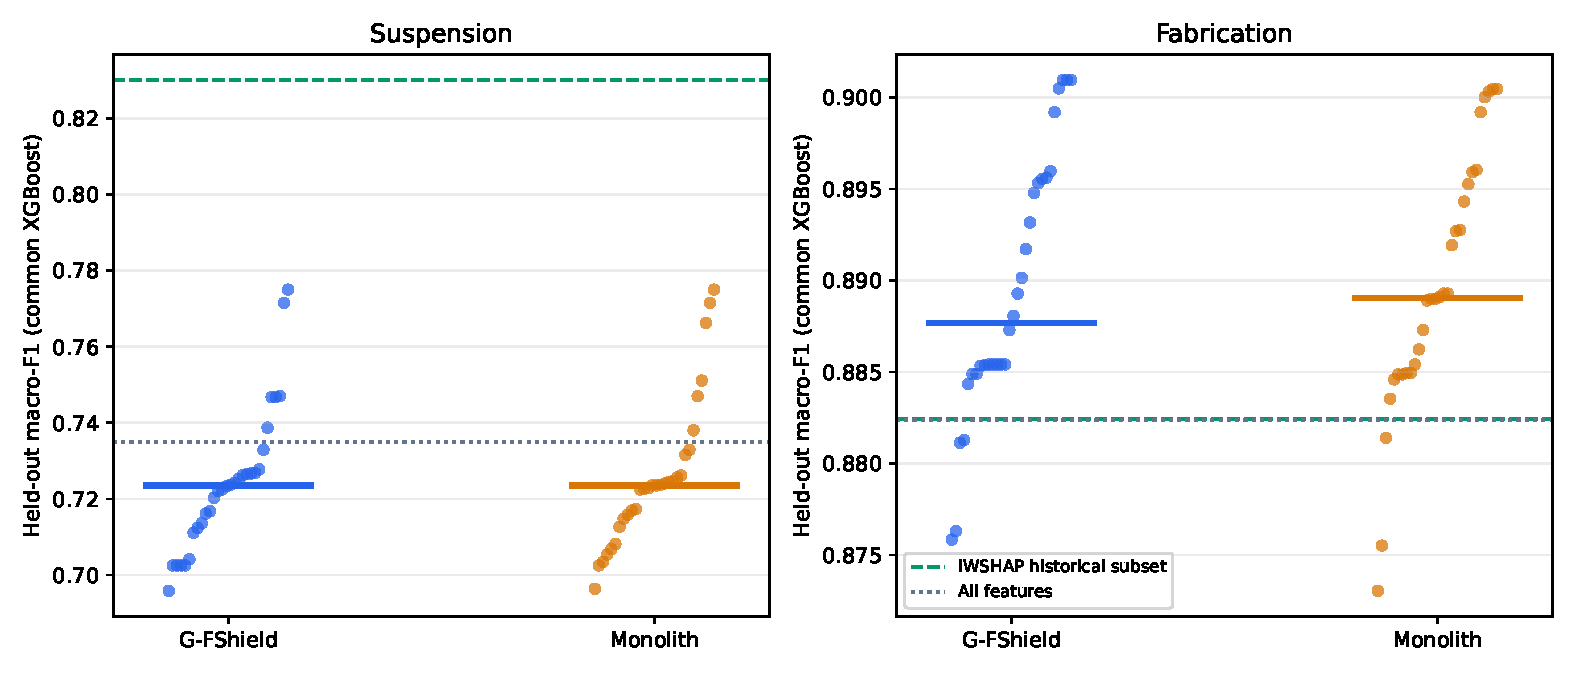
\includegraphics[width=.96\linewidth,height=.80\textheight,keepaspectratio]{fig/gfshield/iwshap-xgboost-common-comparison.pdf}
  \caption{F1 macro dos subconjuntos congelados sob o protocolo XGBoost comum. Traços horizontais mostram os comparadores fixos com todos os atributos e com os atributos do log histórico IWSHAP.}
  \label{fig:iwshap-xgboost}
\end{figure}
\end{landscape}
